\documentclass[12pt, a4paper]{article}
\usepackage[francais]{babel}
\usepackage{caption}
\usepackage{graphicx}
\usepackage[T1]{fontenc}
\usepackage{listings}
\usepackage{geometry}
\usepackage{amsmath}
\usepackage{listings}
\usepackage[colorlinks=true,linkcolor=black,anchorcolor=black,citecolor=black,filecolor=black,menucolor=black,runcolor=black,urlcolor=black]{hyperref}

% \usepackage{mathpazo} --> Police à utiliser lors de rapports plus sérieux

\usepackage{fancyhdr}
\pagestyle{fancy}
\lhead{}
\rhead{}
\chead{}
\rfoot{\thepage}
\lfoot{Martin Baumgaertner}
\cfoot{}

\renewcommand{\headrulewidth}{0.4pt}
\renewcommand{\footrulewidth}{0.4pt}

\begin{document}
\begin{titlepage}
	\newcommand{\HRule}{\rule{\linewidth}{0.5mm}} 
	\center 
	\textsc{\LARGE iut de colmar}\\[6.5cm] 
	\textsc{\Large R405 Automatisation des tâches}\\[0.5cm] 
	\textsc{\large Année 2022-23}\\[0.5cm]
	\HRule\\[0.75cm]
	{\huge\bfseries TP 1 : Objet WMI}\\[0.4cm]
	\HRule\\[1.5cm]
	\textsc{\large martin baumgaertner}\\[6.5cm] 

	\vfill\vfill\vfill
	{\large\today} 
	\vfill
\end{titlepage}
\newpage
\tableofcontents
\newpage
\section{Windows Management Instrumentation}
\subsection{Exercice 1 - Quelle commande permet d’obtenir les instances des classes WMI ?}

La commande qui permet d'obtenir les instances des classes WMI est : 
\textbf{Get-WmiObject -List}

\subsection{Exercice 2 - Combien d’instances sont disponibles ?}
Pour savoir combien d'instances sont disponibles j'ai tout simplement fait la même 
commande que précédemment mais en ajoutant le paramètre \textbf{ | Measure-Object}
ce qui donne : \textbf{Get-WmiObject -List | Measure-Object}
La commande me plusieurs options, dont \textbf{Count : 1182}. Il y a donc 1182
instances disponibles.

\subsection{Exercice 3 - Stockez le résultat de la commande Get-WmiObject -Class Win32\_LogicalDisk...}

Pour stocker le résultat de cette commande j'ai utilisé la commande suivante : 
\textbf{\$disks = Get-WmiObject -Class Win32\_LogicalDisk}, suite à ça, la 
commande est stocké dans la variable \textbf{\$disks}\\

Ensuite, pour afficher toutes les variables du tableau il suffit de faire la
commande suivante : \textbf{\$disks | Format-List *}

\subsection{Exercice 4 - Comptez le nombre de disques à l’aide d’une commande}

Pour compter le nombre de disques, j'ai fait la commande suivante :
\textbf{\$disks | Measure-Object} qui me donne comme résultat :
\textbf{Count : 3}. Il y a donc 3 disques présents. 

\newpage
\subsection{Exercice 5 - Ecrivez un script qui détermine le nombre d’octets pris sur le disque C}
Pour déterminer le nombre d'octets pris sur le disque C, j'ai crée le script suivant : 

\begin{figure}[h]
    \centering
    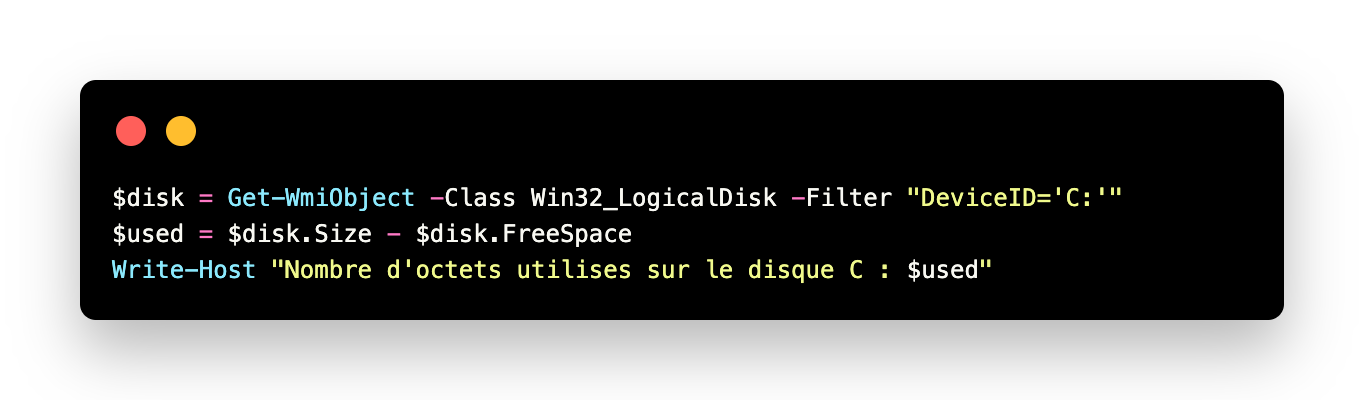
\includegraphics[width=1\textwidth]{img/code1.png}
    \caption{Script 1}
    \label{fig:script1}
\end{figure}

Le script me renvoie ce résultat : \textbf{Nombre d'octets utilises sur le disque C : 18828873728}\\

Premièrement j'ai d'abord stocké dans la variable \textbf{\$disks} le résultat de la commande en filtrant les 
disques qui ont comme nom C. Ensuite, j'ai stocké dans la variable \textbf{\$used} la taille totale du disque C 
en soustrayant l'espace diponible.\\

Enfin, j'ai affiché le résultat de la variable \textbf{\$used}.

\newpage
\subsection{Exercice 6 - Ecrivez un script qui détermine le pourcentage d’occupation du disque C :}
J'ai globalement repris le premier script, j'ai juste le stockage de la variable 
pour la mettre en pourcentage. 
\begin{figure}[h]
    \centering
    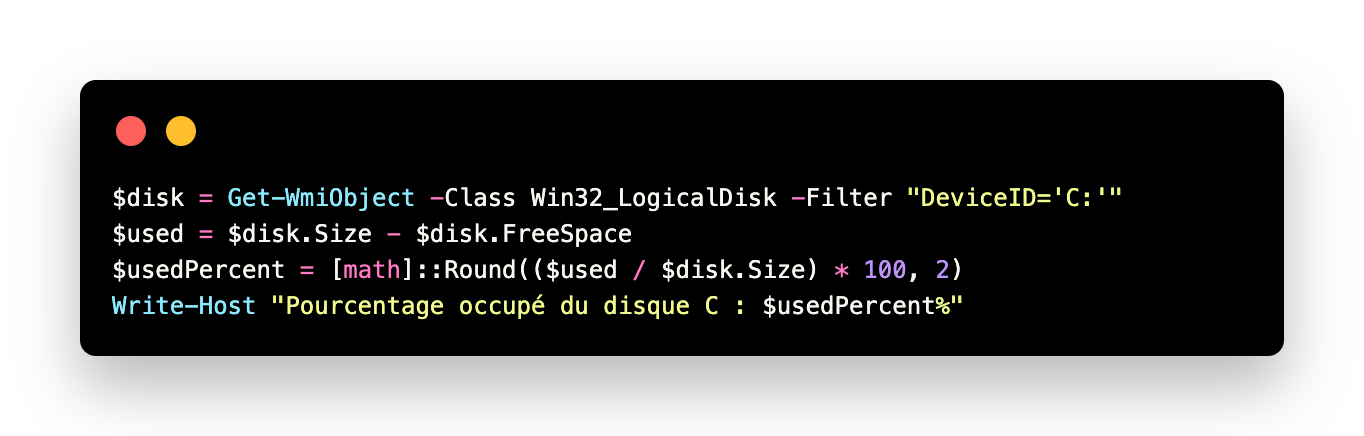
\includegraphics[width=1\textwidth]{img/code2.png}
    \caption{Script 2}
    \label{fig:script2}
\end{figure}

Le script me renvoie le résultat suivant : \textbf{Pourcentage occupé du disque C : 29.38\%}

\subsection{Exercice 7 - Écrivez un script qui détermine le pourcentage d’occupation de chaque disque présent sur la machine.}
\begin{figure}[h]
    \centering
    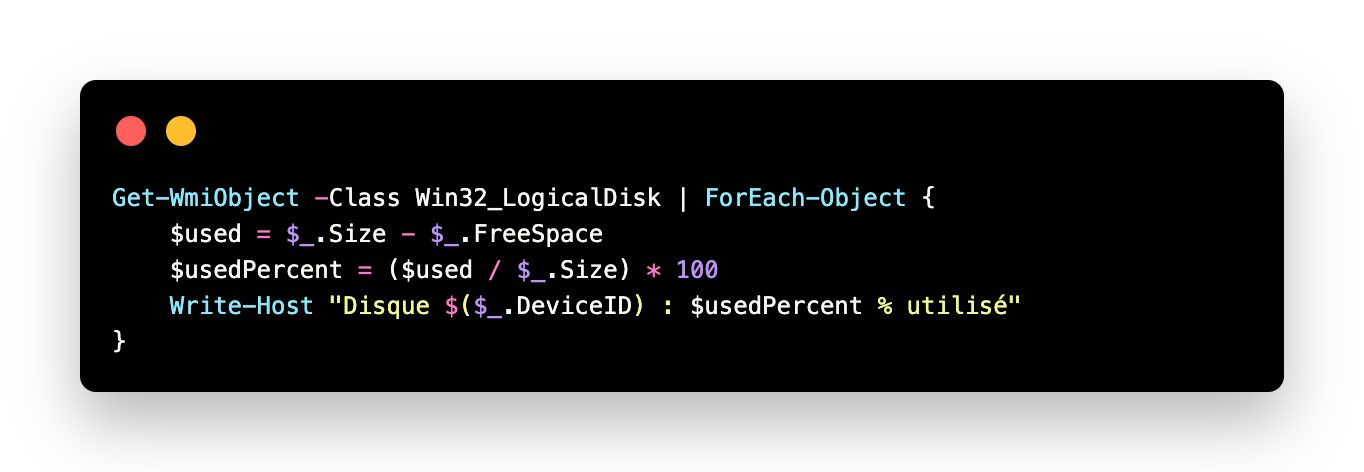
\includegraphics[width=1\textwidth]{img/code3.png}
    \caption{Script 3}
    \label{fig:script3}
\end{figure}
Voici le script pour déterminer le pourcentage d'occupation de chaque disque présent sur la machine.\\

\subsection{Exercice 8 - Vérifier le bon résultat de vos commandes sur la machine Windows de la salle}
Nous obtenons bien le même résultat que la machine hôte windows de la salle. 

\subsection{Exercice 9 - Avec la commande Get-WmiObject -Class ...}
Pour trouver mon adresse IP, avec la commande \textbf{Get-WmiObject -Class Win32\_NetworkAdapterConfiguration}, 
je recherche juste juste le paramètre \textbf{IPAddress} qui me donne comme résultat : \textbf{192.168.197.128}

\subsection{Exercice 10 - Donnez la différence}
La principale différence entre les classes \textbf{WMI Win32\_NetworkAdapter} \\et 
\textbf{Win32\_NetworkAdapterConfiguration} est que la première représente l'adaptateur 
réseau physique, tandis que la seconde représente les paramètres de 
configuration réseau appliqués à l'adaptateur

\subsection{Exercice 11 - Avec l’option ComputerName obtenez le ou les adresses MAC des cartes de votre voisin ?}
Pour faire ceci, il faut écrire la commande suivante :\\
\textbf{Get-NetNeighbor -ComputerName "nom"}

\subsection{Exercice 12 - Que fait la commande Test-Connection ?}
La commande test-connection envoie 4 pings vers la destinations que l'on
souhaite joindre. Par exemple si je fais la commande suivante :
\textbf{Test-Connection google.com}, je vais envoyer 4 pings vers
google.com.\\

\subsection{Exercice 13 - Reprendre la commande précédente pour avoir un résultat binaire}
En rajoutant l'option \textbf{-Quiet}, j'obtiens \textbf{True} si la commande
de ping réussi, et \textbf{False} si elle échoue. On a donc par exemple 
\textbf{Test-Connection google.com -Quiet}

\subsection{Exercice 14}
\subsubsection{Consigne}
Écrivez un script qui prend en paramètre une adresse IP et qui test la 
connexion avec cette machine et qui stocke dans un tableau le nom de la 
machine (Win32\_Desktop)le nom de l’OS, la version et ma clé d’activation 
(Win32\_OperatingSystem). Vous laisserez le choix à l’utilisateur d’afficher 
les résultats ou bien de le stocker dans un fichier csv.

Voici le script que j'ai réalisé. Il permet donc comme demandé de tester la 
connexion, puis on demande a l'utilisateur si on veut exporter les données
dans un fichier csv. Si oui, on demande le nom du fichier, sinon on affiche
les données dans la console.\\

\begin{figure}[h]
    \centering
    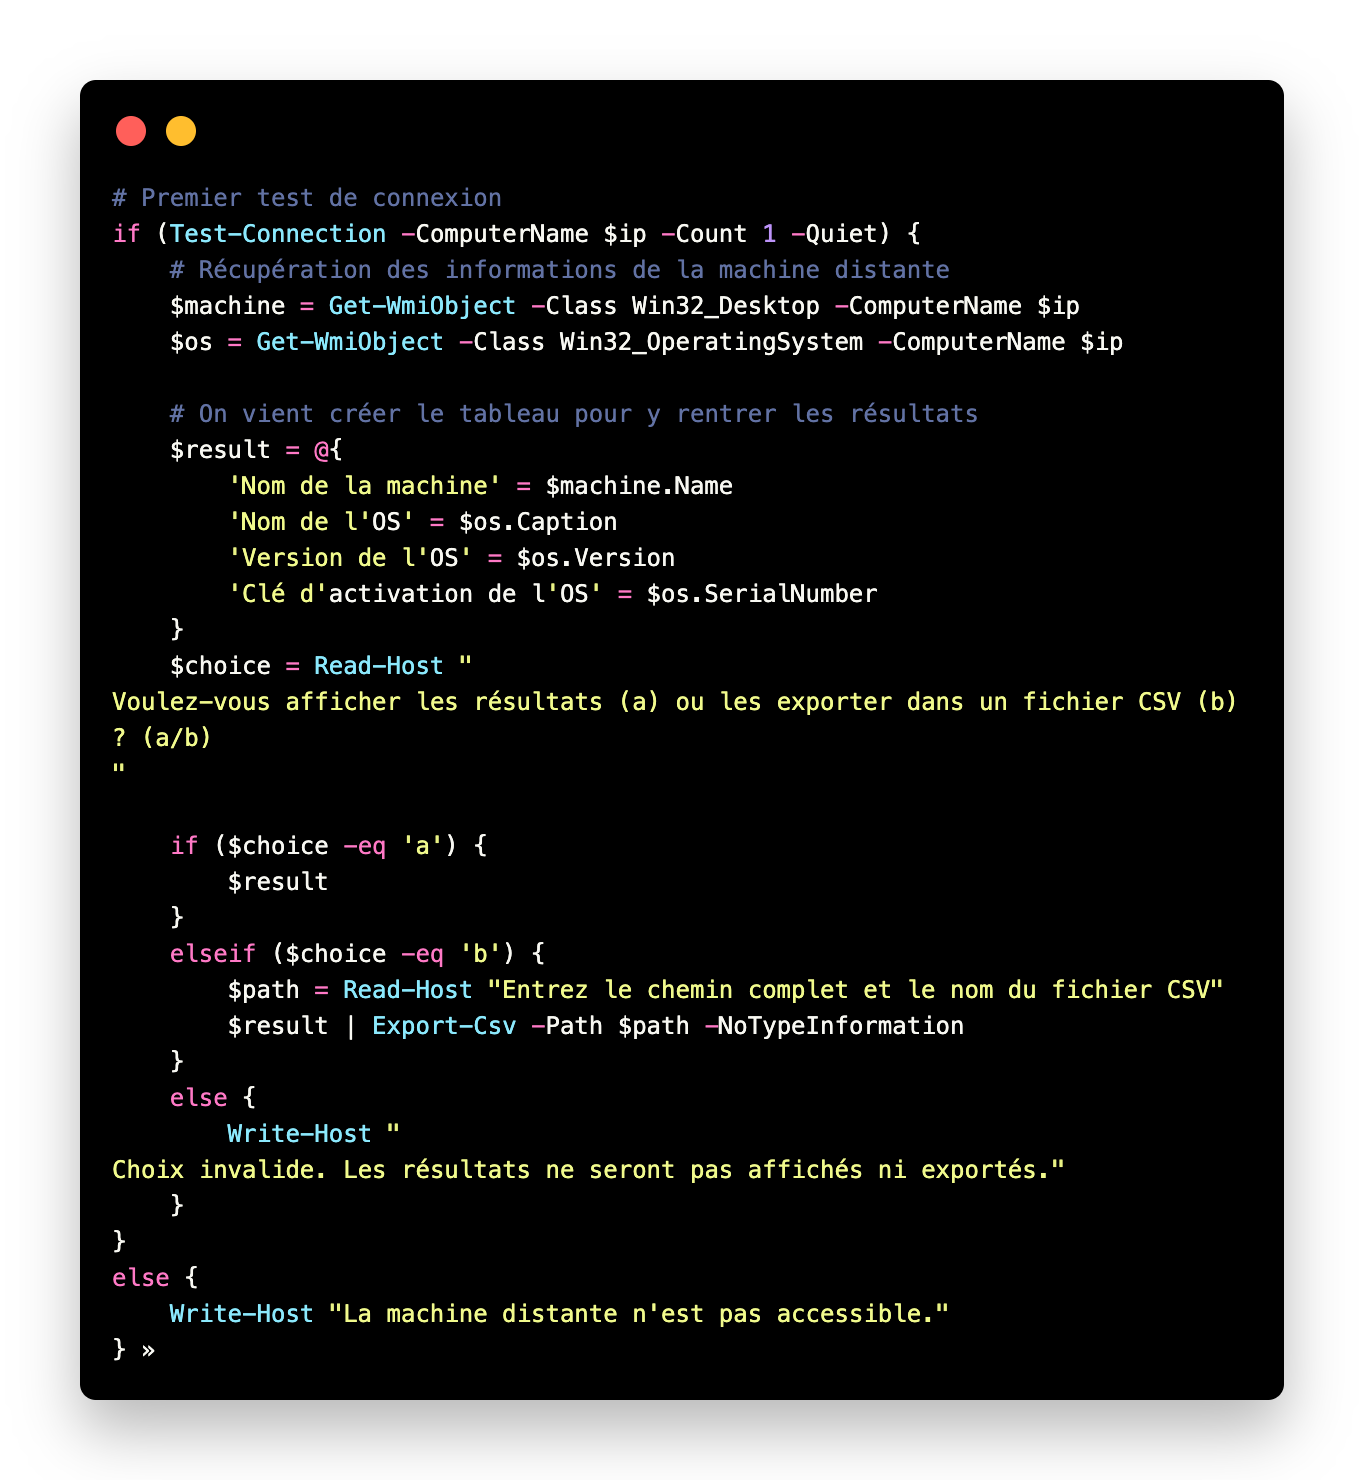
\includegraphics[width=0.8\textwidth]{img/code5.png}
    \caption{Script final}
    \label{fig:script-final}
\end{figure}



\subsection{Question Bonus - A quoi correspond FAT32}
FAT32 correspond tout simplement au bootloader de Windows.


\end{document}